
\sloppy
%----------------------------------------------------------------------------------------
% Section 2.1 (overview)
%----------------------------------------------------------------------------------------

\section{Overview}

Overview section goes here.

\newpage

%----------------------------------------------------------------------------------------
% Section 2.2 Research work goes here
%----------------------------------------------------------------------------------------

\begin{refsection} % This handles the references independently

\section{Section name}
\label{section:2.2} % This is used to cross reference internally

Here goes all the text presenting the work.
Here goes an example reference \parencite{Fierer2014,Sunagawa2015}.
Here goes an example equation: \\

\begin{equation}
Trait_{real} = \frac{1}{total\_abund} \sum_{i=1}^{k} genome\_trait_i \times genome\_abund_i
\label{eq:2.3-6}
\end{equation}
\vspace{0.5cm}

%----------------------------------------------------------------------------------------
% Bibliography
%----------------------------------------------------------------------------------------
\clearpage
\pagestyle{plain}
\printbibliography
\end{refsection}
\clearpage
\pagestyle{fancy}

%----------------------------------------------------------------------------------------
% Figures
%----------------------------------------------------------------------------------------

\newpage

\textbf{Figures}

\begin{figure}[h]
\centering
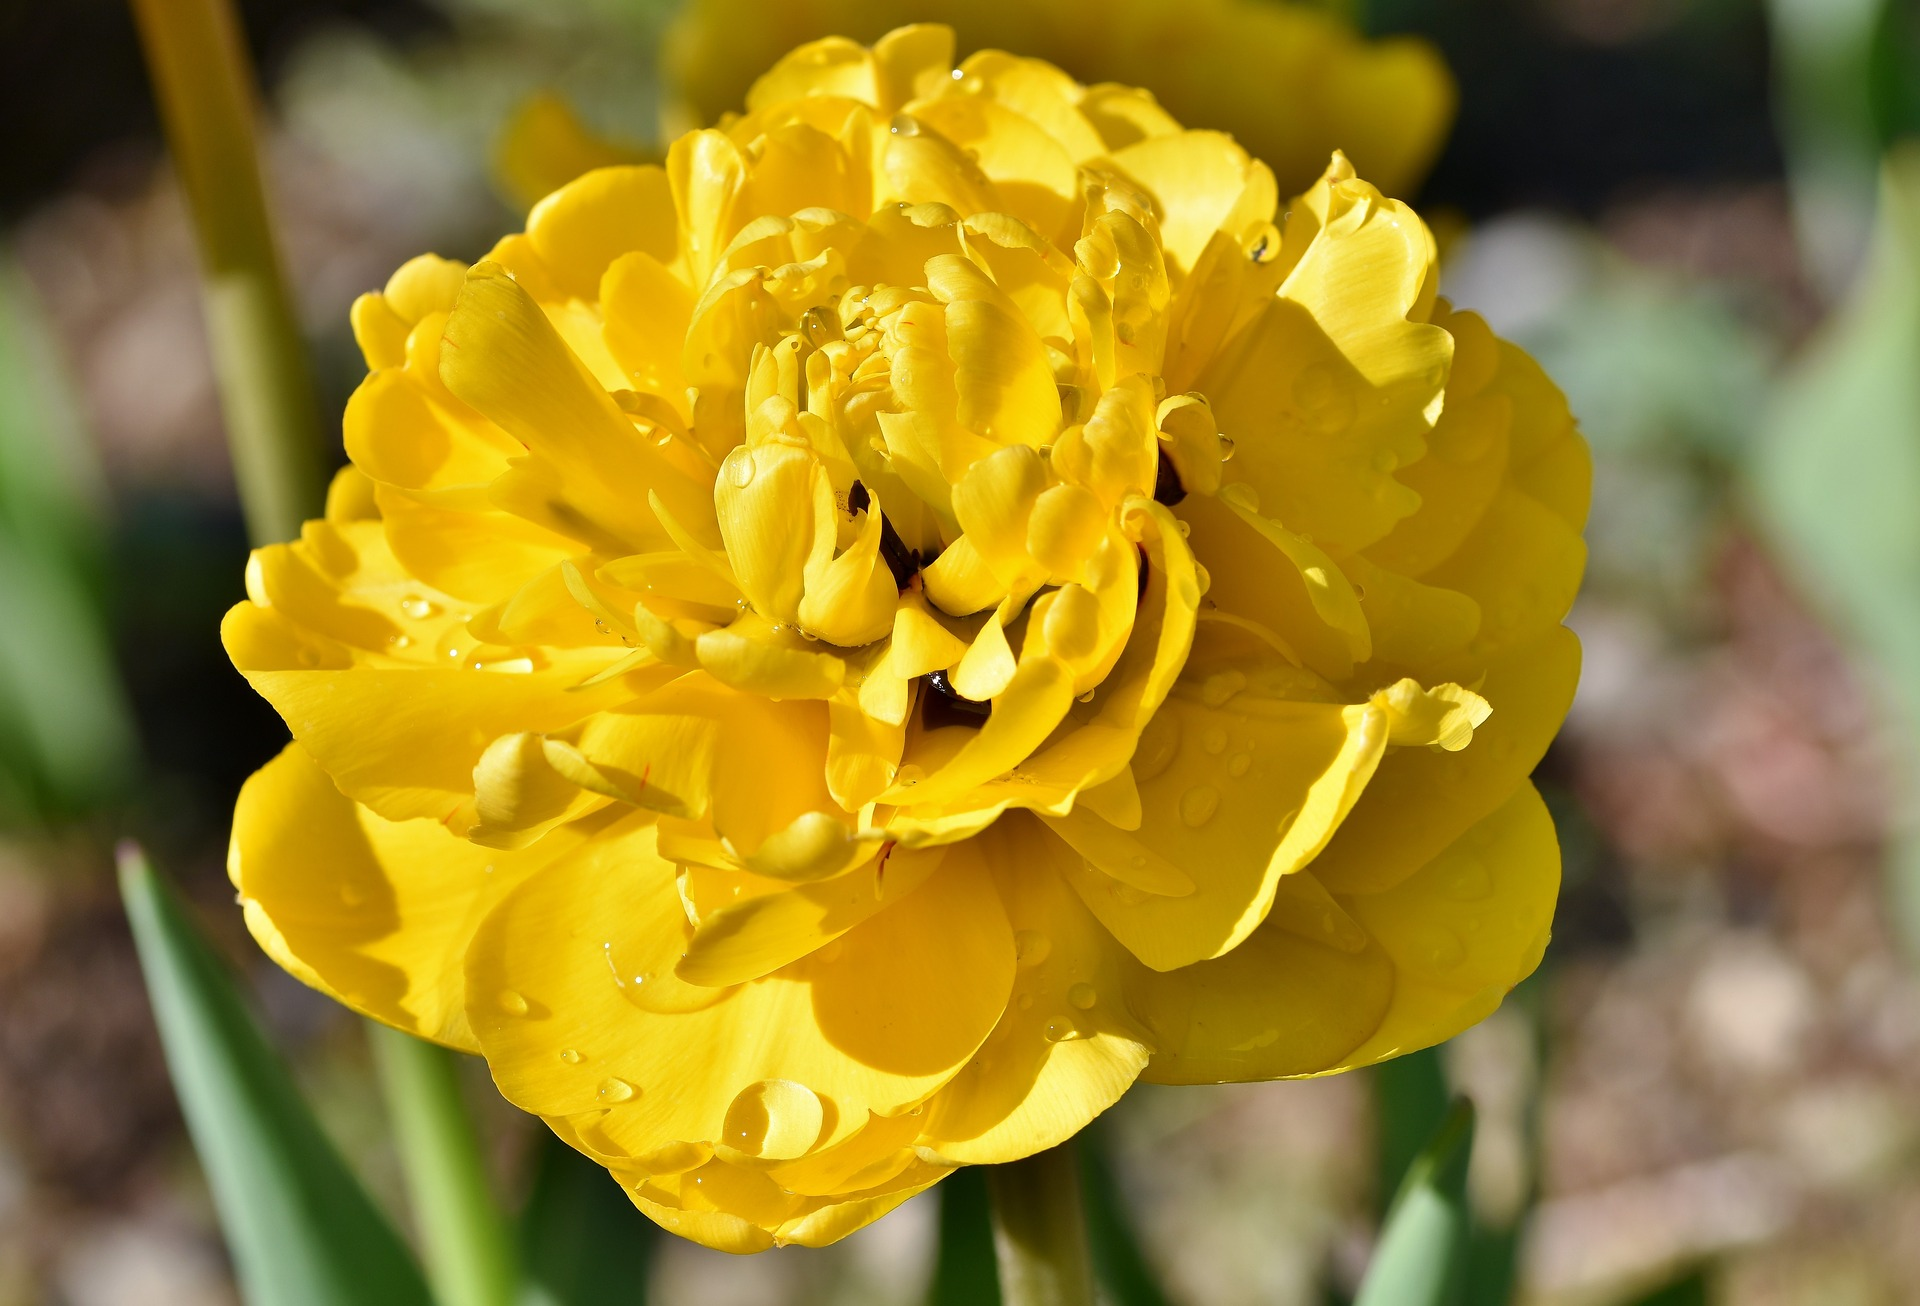
\includegraphics[scale=0.5]{chapter_2.2_figures/fig_2_2_1.jpg}
\setstretch{1.5}
\caption{\textbf{Figure name} \textbf{1)} Figure caption}
\label{fig:2.2-1}
\end{figure}


%----------------------------------------------------------------------------------------
% Table 
%----------------------------------------------------------------------------------------

\newpage

\begin{table}[h]
\setstretch{1.5}
\centering
\caption{\textbf{Multi-valued traits summary variables.} Details of the first principal components (PC1) obtained from the Principal Component Analysis (PCA) performed on the multi-valued traits.}
\begin{scriptsize}
\begin{tabular}{l c c c}
\hline
\textbf{Field1} & \textbf{Field2} & \textbf{Field3} \\
 \hline
sometext & somevalue & somevalue\\
sometext & somevalue & somevalue\\
sometext & somevalue & somevalue\\
sometext & somevalue & somevalue\\
sometext & somevalue & somevalue\\
sometext & somevalue & somevalue\\
\hline
\end{tabular}
\end{scriptsize}
\label{table:2.2-1}
\end{table}

